
\chapter{Neuroadaptive Technology Enables Implicit Cursor Control Based on Medial Prefrontal Cortex Activity}
\chaptermark{Neuroadaptive Technology Enables Implicit Cursor Control}%
\label{chapter:nat}%


{\chaptermeta

\textbf{Zander, T. O.\textsuperscript{1,2,*}, Krol, L. R.\textsuperscript{1,2,*}, Birbaumer, Niels\textsuperscript{3,4}, \& Gramann, K.\textsuperscript{1,5}}

{\small
\textsuperscript{1}Biological Psychology and Neuroergonomics, Technische Universität Berlin, Berlin, Germany
\textsuperscript{2}Team PhyPA, Technische Universität Berlin, Berlin, Germany
\textsuperscript{3}Institute for Medical Psychology and Behavioural Neurobiology, University Tübingen, Tübingen, Germany
\textsuperscript{4}Wyss Center for Bio and Neuroengineering, Geneva, Switzerland
\textsuperscript{5}Center for Advanced Neurological Engineering,
University of California San Diego, San Diego, USA \textsuperscript{*}Shared first authorship

This is the postprint version of the manuscript published as follows:

Zander, T. O., Krol, L. R., Birbaumer, N. P., \& Gramann, K. (2016). Neuroadaptive technology enables implicit cursor control based on medial prefrontal cortex activity. \emph{Proceedings of the National Academy of Sciences, 113}(52), 14898–14903. doi: 10.1073/pnas.1605155114\nocite{zander2016nat}
\par}}


\abstract%
The effectiveness of today' s human–machine interaction is limited by a communication bottleneck as operators are required to translate high-level concepts into a machine-mandated sequence of instructions. In contrast, we demonstrate effective, goal-oriented control of a computer system without any form of explicit communication from the human operator. Instead, the system generated the necessary input itself, based on real-time analysis of brain activity. Specific brain responses were evoked by violating the operators' expectations to varying degrees. The evoked brain activity demonstrated detectable differences reflecting congruency with or deviations from the operators' expectations. Real-time analysis of this activity was used to build a user model of those expectations, thus representing the optimal (expected) state as perceived by the operator. Based on this model, which was continuously updated, the computer automatically adapted itself to the expectations of its operator. Further analyses showed this evoked activity to originate from the medial prefrontal cortex and to exhibit a linear correspondence to the degree of expectation violation. These findings extend our understanding of human predictive coding and provide evidence that the information used to generate the user model is task-specific and reflects goal congruency. This paper demonstrates a form of interaction without any explicit input by the operator, enabling computer systems to become neuroadaptive, that is, to automatically adapt to specific aspects of their operator' s mindset. Neuroadaptive technology significantly widens the communication bottleneck and has the potential to fundamentally change the way we interact with technology.


\clearpage


\fancypagestyle{nat}{%
    \fancyhf{}
    \fancyhead[EC]{\textit{\leftmark}}
    \fancyhead[OC]{\textit{\rightmark}}
    \fancyfoot[C]{\thepage \\ \vspace{6.8mm} \colorbox{footerbg}{\parbox{\paperwidth-2\fboxsep}{\centering\parbox{0.75\paperwidth}{\centering\fontsize{9pt}{9pt}\selectfont\textcolor{footerfg}{This is the postprint version of published manuscript: Zander, T. O., Krol, L. R., Birbaumer, N. P., \& Gramann, K. (2016). Neuroadaptive technology enables implicit cursor control based on medial prefrontal cortex activity. \emph{Proceedings of the National Academy of Sciences, 113}(52), 14898–14903.}}}}}
    \fancyfootoffset[]{1.25in}}
\pagestyle{nat}


\section{Significance}
The human brain continuously and automatically processes information concerning its internal and external context. We demonstrate the elicitation and subsequent detection and decoding of such ``automatic interpretations'' by means of context-sensitive probes in an ongoing human–computer interaction. Through a sequence of such probe-interpretation cycles, the computer accumulates responses over time to model the operator' s cognition, even without that person being aware of it. This brings human cognition directly into the human–computer interaction loop, expanding traditional notions of ``interaction.'' The concept introduces neuroadaptive technology---technology which automatically adapts to an estimate of its operator' s mindset. This technology bears relevance to autoadaptive experimental designs, and opens up paradigm-shifting possibilities for human–machine systems in general.


\section{Introduction}

In the European Union, 96\% of enterprises rely on computers for their productivity \cite{eurostatisoc_ci_eu_en2}. Advances in human-computer interaction (HCI), concerning the effective, efficient, and satisfying use of computer systems, may thus carry great societal benefits, e.g. in terms of productivity \cite{rogers2011}. However, although interaction techniques have become increasingly user-friendly---e.g. from punch cards to touch screens---they still depend on the user (operator) to translate their original thought or intention into a sequence of small, explicit commands. This translational step, where the human operator must ultimately obey the machine's logic, presents both a communication bottleneck and a source of potential error \cite{tufte1990}. At the same time, the computer has practically no limitation to the amount of information it can communicate, and is not as adaptable as its user. In these aspects, present-day HCI is asymmetrical \cite{suchman1987hmcproblems}. Comparing this to human-human interaction, \citeA{fischer2001usermodeling} emphasizes the importance of a shared understanding of the situation and an understanding of the communication partner. In this sense, for a computer system to `understand' its user, it needs a model of that user---a source of information that goes beyond the explicitly given commands. On the basis of such a model, a computer system could adapt its behavior to better suit the current mode of the user \cite{fischer2001usermodeling}. This could help alleviate the issue of asymmetry. Relevant information to that end concerns the user's intentions, subjective interpretations, and emotions. 

Four decades of developments in brain–computer interfaces (BCIs) \cite{vidal1973direct,wolpaw2012bcibook} have yielded a set of methods that may be used to obtain such information in real time, provided that this information is detectably reflected in brain activity. Specifically, BCIs can detect in real time changes in the electroencephalogram (EEG) and translate these changes into control signals, in line with the principles of physiological computing \cite{fairclough2009fundamentals}. A subgroup of BCIs, so-called ``passive BCIs'' (pBCIs) \cite{zander2011}, focuses on monitoring otherwise covert aspects of the user state \cite{zander2012context} during an ongoing HCI. Neurophysiological correlates of the above-mentioned aspects can be detected and interpreted in the context of the interaction, and can be used to inform the computer about relevant changes in the user's cognition and affect. Using pBCI, thus, a computer can in fact acquire information about its operator other than the explicitly given commands. As such, neurophysiological activity can induce appropriate changes in the machine in real time, essentially serving as an implicit command, without requiring the user to exert any conscious effort in communicating to the computer \cite{zander2011}.

Previous and present-day BCI systems use information derived about the user state in only an ad hoc fashion: momentary information derived by the BCI from the EEG is directly interpreted as a specific user intention \cite{schultzekraft2016veto,zander2010gazeinput}, situational interpretation \cite{blankertz2011}, or a change in the cognitive \cite{gerjets2014workload} or affective \cite{chanel2009emotion} state. These implementations represent one-to-one mappings of user states to machine behavior. We propose, however, that a machine using pBCI can detect both general user states and transient, event-related responses, and can use these to continuously and accumulatively learn about its operator. Specifically, we propose that the machine collates the neurophysiological responses of its operator (i.e., implicit inputs) and coregisters them against the events and contexts that evoked them. This allows the machine to build and continuously update a specific and context-sensitive model of that operator \cite{zander2012context}. The goal is to combine the information gathered from multiple responses to different events to gain insights into higher-level aspects of the operator's cognition.

One aspect of higher cognition that may be inferred in this manner is described by the theory of human predictive coding. Predictive coding holds that there exists a continuous, automatic prediction of future (neuronal) events, as well as a continuous comparison of those predictions with their corresponding final perception \cite{clark2013predictive,friston2010free,brown2011inference}. Discrepancies resulting from these comparisons inform the brain of the correctness of its predictions and actions, providing a fundamental mechanism---prediction error minimization---to shape and optimize behavior. The corresponding predictive signals are assumed to be carried by the dopaminergic system. Changes in the continuous evaluation of events and actions lead to changes in the dopaminergic input to the anterior cingulate cortex, (dis)inhibiting its neurons and eliciting a detectable response \cite{holroyd2002}. Predictions of what is expected to happen, in this sense, relate closely to what is intended to happen. This makes the correlates of predictive coding a fundamental source of information concerning user intention---an aspect of the user's cognition that is highly relevant to HCI.

In this paper, we demonstrate that by collating passive BCI output and context information, it is possible to develop, step by step, a user model that accurately reflects correlates of predictive coding and reveals task-relevant subjective intent.

Specifically, we demonstrate that a user model can be developed and used to guide a computer cursor toward the intended target, without participants being aware of having communicated any such information. Using a passive BCI system, the participant's situational interpretations of cursor movements were classified and interpreted, in the given context, as directional preferences. A user model was generated to represent these context-dependent directional preferences, and this model was then used to guide the cursor toward the intended movement direction.


\section{Results}

The experimental paradigm involved a form of cursor control. The cursor moved discretely over the nodes of a (4$\times$4 or in later stages 6$\times$6) grid. For each movement the cursor could travel up to eight directions, horizontally, vertically, and diagonally, to one of the adjacent nodes. Each movement served both to move the cursor and to elicit a neurophysiological response, reflecting the subjective correctness of that movement. In essence, each movement thus also served as a probe for information. One of the grid's corners was designated the target. For each movement, it could thus be determined at what angle of deviance relative to the target the cursor had moved. This was used for an objective interpretation of the cursor's behavior. We describe the paradigm in detail in SI Appendix.

The event-related potential (ERP) following each probe (i.e., each cursor movement) is shown in Fig. \ref{fig:nat:figure1}\emph{a}. A one-way analysis of variance of the systematic peak differences around 180 ms indicated a significant main effect of angular deviance from the target direction on peak amplitude [\textit{F}(7,126) = 47.243, \textit{P} < 0.001]. Specifically, the peak amplitudes (Fig. \ref{fig:nat:figure1}\emph{b}, upper curve) differed significantly (\textit{P} < 0.001) between both the lowest and the highest angular deviation from the target direction as used by the classifier. In between, the peak amplitudes scaled linearly with angular deviance, as fitted by a linear regression model using each group's mean angular deviance as a predictor (slope coefficient \textit{b} = −0.0035, \textit{F} = 45.28, \textit{P} < 0.001; \textit{R$^{2}$} = 0.33). Further posthoc comparisons corrected for false discovery rate additionally indicated that significant differences between adjacent groups (\textit{P} < 0.05) were found mostly for groups of lower angular deviance, whereas differences between the three largest-deviance groups (124$^{\circ}$ and up) were not significant. The results of all posthoc comparisons are listed in SI Appendix, Table S3. In summary, the probe elicited systematic variations in event-related amplitudes, depending on the goal congruency of the presented stimulus.

\begin{figure}[ht]
    \centering
    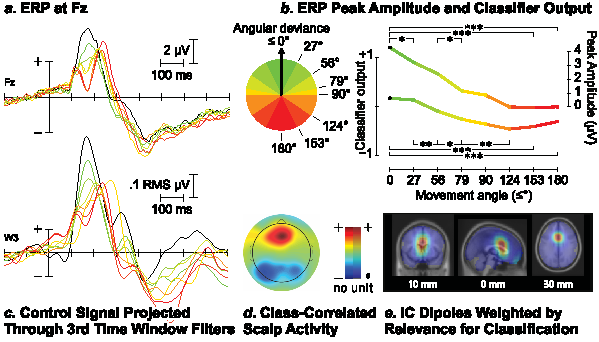
\includegraphics[width=\textwidth]{figures/nat-figure1.pdf}
    \caption[Neurophysiological analysis.]{Neurophysiological analysis. (a) Grand average ERP at Fz (\textit{n} = 19) time-locked to cursor movement, divided into eight groups depending on angular deviance. (b) Peak amplitudes around 180 ms for the ERP in A, and mean classifier output for cursor movements sorted by angular deviance with selected significant differences indicated (\textit{***P} < 0.001, \textit{**P} < 0.01, \textit{*P} < 0.05). (c) Grand average ERP (\textit{n} = 19) projected through the sources focused on in the third time window (150–200 ms; indicated in gray). (d) Scalp map of difference-between-classes activity that contributed to classification in the third time window. (e) Source localization for the third time window.}
    \label{fig:nat:figure1}
\end{figure}

To enable real-time detection of the individual, single-trial neuroelectric responses, we calibrated a discriminative classification system. Calibration was based on two classes of responses representing the extreme ends of the spectrum, with angular deviances of 0$^{\circ}$ making up the one class, and angular deviances of ≥135$^{\circ}$ the other (Fig. \ref{fig:nat:figure2}\emph{a}). This classification system used a subject-dependent linear combination of all 64 available channels, taking into account full scalp information. It automatically generated appropriate spatial filters for eight 50-ms time windows---starting at 50 ms after stimulus presentation---using supervised machine learning and linear discriminant analysis. This set of filters weighted each electrode in each time window, depending on its relevance to classification. The recorded signal projected through them thus allowed an optimal discrimination between the two classes. This projected recorded signal---from all 64 channels, between 50 and 450 ms after stimulus presentation---defined the control signal. The feature extraction is described in more detail in SI Appendix.


\begin{figure}[ht]
    \centering
    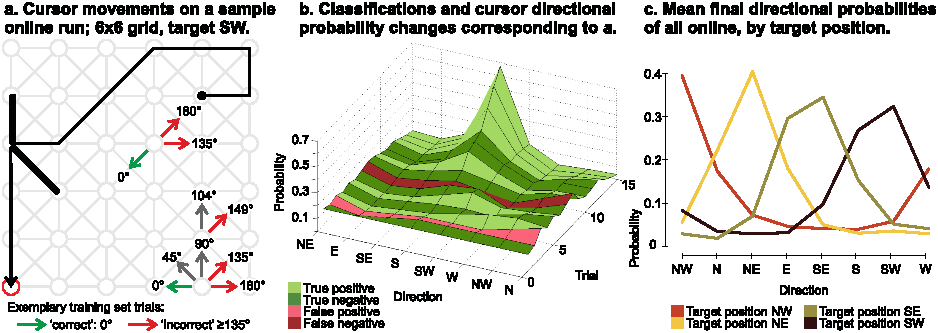
\includegraphics[width=\textwidth]{figures/nat-figure2.pdf}
    \caption[Cursor behavior and user model generation.]{Cursor behavior and user model generation. (a) Sample online cursor movements. Also indicated: selected movement directions, their relative angular deviance, and class membership (calibration phase). Movements with an angular deviance >0$^{\circ}$, <135$^{\circ}$ (e.g., gray arrows) were not in the training set. (b) User model evolution during the movements in A based on movement classifications. Ground truth is taken from button presses. (c) The mean final user model representing the directional probabilities/preferences upon reaching the target, grouped by absolute target position.}
    \label{fig:nat:figure2}
\end{figure}

The resulting classification system not only provided a filtered discriminative control signal; it also allowed us to investigate which cortical sources the system focused on. Based on this information, conclusions can be drawn about the discriminative cognitive processes underlying the classification. Fig. \ref{fig:nat:figure1}\emph{c–e} shows an analysis of the features used for classification between 150 and 200 ms, highlighting the relevant factors in this time window: the discriminative scalp activity, the source localization of this activity within the brain, and a projected ERP of the signal generated from the identified sources. SI Appendix, Fig. S5 and Movies S1 and S2 present this same analysis for the full time course under investigation. See SI Appendix, Fig. S8 for scalp maps of the class-specific activity in each time window.

This approach identified a specific neuroanatomical area across participants: The system based its decisions on neuronal activity that predominantly originated in the medial prefrontal cortex (mPFC). The classification system was trained only on two binary classes representing the smallest and largest angular deviances. Back-projection of the signal through the system's filters, however, reveals that the classification system optimally identified the same sources that generated the linear modulations seen in the grand average ERP. Following the pattern found for the peak amplitudes at Fz, peak amplitudes of the projected ERPs differed significantly (\textit{P} < 0.001) between the classes used by the classifier. In between, the peak amplitudes scaled linearly with angular deviance, as fitted by a linear regression model of the aggregated means, using each group's mean angular deviance as a predictor (\textit{b} = −0.0019, \textit{F} = 31.9, \textit{P} = 0.011; \textit{R$^{2}$} = 0.91). Statistically significant differences between adjacent groups also followed a similar pattern; see SI Appendix, Table S5 for all pairwise comparisons. It is thus clear that the classification system focused on a response that reflected the probe's logic.

The signal thus carried task-relevant information. For a true test of this signal's single-trial reflection of individual judgments of cursor movements, and thus its usefulness in creating a user model describing subjective intent, we created a closed-loop, online version of the original offline paradigm. Following each single cursor movement, an individually calibrated classification system classified the evoked response. The extracted information was used for reinforcement learning on the side of the cursor \cite{sutton1998reinforcementlearning}, modifying the probabilities of upcoming cursor movements such that the cursor would be more likely to go toward the target if the classifications were correct. The resulting probability statistics can then be understood as a user model, describing the user's preferred behavior of the cursor. This description's accuracy is then reflected in the user model's success in enabling effective, goal-oriented control of the cursor.

Performance was operationalized as the number of cursor movements required to reach one target. Because even a completely randomly moving cursor would eventually reach the target, three conditions were distinguished: random, online, and ``perfect.'' In the random condition, no reinforcement took place and the cursor merely moved randomly. In the online condition, the cursor was reinforced based on the classifications of the classification system. The perfect condition was simulated: the cursor already knew the location of the target and reinforced itself with 100\% accuracy, although it did proceed to move probabilistically. This condition represents the best possible performance given the constraints of the grid and the cursor's movement algorithm.

The offline calibration data were gathered on a 4$\times$4 grid. The online, closed-loop system was tested on both a 4$\times$4 grid, and on a theretofore unseen 6$\times$6 grid. Performance results are summarized in Fig. \ref{fig:nat:figure3}.

\begin{figure}[ht]
    \centering
    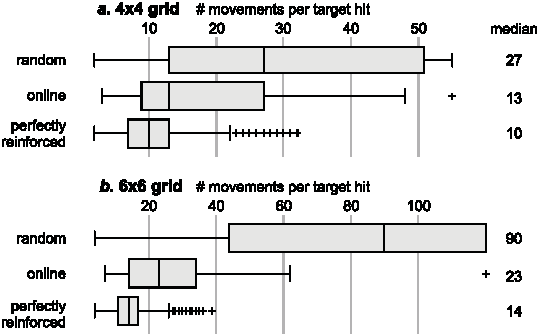
\includegraphics[width=0.64\textwidth]{figures/nat-figure3.pdf}
    \caption[Performance measure distributions for nonsupported, online, and perfectly reinforced cursor movements on the two online grid sizes.]{Performance measure distributions for nonsupported, online, and perfectly reinforced cursor movements on the two online grid sizes. (a) Performance on the 4$\times$4 grids. (b) Performance on the 6$\times$6 grids. All differences between the three conditions are significant (\textit{P} < 0.025). Whiskers cover $\pm$2.7$\sigma$.}
    \label{fig:nat:figure3}
\end{figure}

On the 4$\times$4 grid, a randomly moving cursor required an average of 27 movements. In the simulated condition of perfect performance, this number dropped to 10. When the cursor was reinforced online, an average of 13 steps was required---a significant improvement compared to the random condition (\textit{P} < 0.025) bridging the gap toward the perfect condition by 82\%.

On the 6$\times$6 grid random cursor movement required 90 steps on average, and 14 in the perfect-accuracy simulation. Even though no training data had been gathered from the 6$\times$6 grids, the online system bridged this gap by 88\%, requiring 23 movements on average (\textit{P} < 0.01).

On both grids, the online performance also differed significantly from the perfect performance (\textit{P} < 0.025).

Movie S3 shows a number of online cursor movements and illustrates the adaptive paradigm's responses.

Online application thus significantly increased the goal congruency, confirming that the signal the classification system focused on was situationally relevant. Although the cursor only made binary interpretations of the classifier's output, this output was continuous: a scale, from −1 to +1, correlating to the movements' degree of goal congruency. This is illustrated in Fig. \ref{fig:nat:figure1}\emph{b} (lower curve). The classifier output differs significantly (\textit{P} < 0.001) between the classes used by the classifier. In between, the classifier output scaled linearly with angular deviance, as fitted by a linear regression model using each group's mean angular deviance as predictor (\textit{b} = 0.0035, \textit{F} = 295.42, \textit{P} < 0.001; \textit{R$^{2}$} = 0.76). See SI Appendix, Table S4 for further comparisons.

Even though the linearly scaled information was not taken into account, binary classifications still resulted in a graded user model, describing the appropriateness of the different cursor movements depending on the intended target's position. To illustrate this, Fig. \ref{fig:nat:figure2}\emph{a} visualizes the cursor's movements over a grid during one of the online runs with the target in the southwest corner. Fig. \ref{fig:nat:figure2}\emph{b} shows how the individual directional preferences/probabilities in the user model are updated after every cursor movement, showing the progression toward a clearly identified preference for the southwest corner. Fig. \ref{fig:nat:figure2}\emph{c} illustrates the mean final user models for all participants for the four different target positions. It is clear that the user models accurately represent the intended target position. The mean final user model across all participants is illustrated in SI Appendix, Fig. S4, with statistics in SI Appendix, Table S2. SI Appendix, Fig. S9 shows one more example of online cursor behavior.


\section{Discussion}

We have demonstrated that binary classifications of subjective interpretations of cursor movements can be aggregated into a user model reflecting, in the given context, directional intent. Based on this model, the cursor was effectively guided toward the target. Participants were not aware of their influence on the cursor. Although not used explicitly in this study, analysis shows that more fine-grained information may be available in the elicited responses, encoded in the linear dependency of the response on the angular deviance.

An approach combining independent component analysis (ICA, \citeNP{bell1995,makeig1996}), supervised machine learning, and higher-order statistics not only gave insight into the individual single-trial responses, but also enabled error-minimized source localization and signal back-projection as well as real-time single-trial analysis. These characteristics could be used to validate the classification system as well as the user model. Firstly, the online application of the classification system increased the paradigm's goal congruency to near the optimum: The gap from no reinforcement to optimal reinforcement could be bridged by over 80\% using the presented classification system, both on the 4$\times$4 grid and on the theretofore unseen 6$\times$6 grid. This significant reduction in the number of steps required to reach a target provides evidence that the classification of brain responses following a cursor movement was based on task-relevant information: Each movement indeed elicited a response enabling the identification of subjective directional preferences.

Secondly, the neurophysiological analysis, based on the classification system's filter set, revealed that the underlying signal predominantly stemmed from the mPFC, and reflected the experimental paradigm's logic. Further interpretation of the neurophysiological response points to its likely generator process. Given the signal's time course, its localization, and the evoking stimuli, the response is in line with the framework of predictive coding. We hypothesize that in the present study, participants consistently predicted---for lack of information that would indicate otherwise---that the cursor would perform the only action that would have been appropriate, i.e., that it would move in the direction of the target. Interestingly, however, our findings imply an extension of the general framework of predictive coding. A focus on ``negative'' signals is central to current interpretations and findings related to predictive coding: Indications of discrepancies, of prediction errors, are seen as central to learning by reinforcement, in turn explaining the large range of rich human behavior and intelligence \cite{hawkins2004intelligence}. The sensitivity of the ERP amplitude to the quality of the cursor movements, however, seems to indicate that neural activity generated within the mPFC provides a range of graded responses to both positive and negative movements. In this context, these reflect the observer's directional preferences, modeling an important, task-relevant factor of their subjective cognition. This points to a continuous response range within the mPFC that not only detects deviations from a predicted event to adapt future behavior, but also confirms correct predictions to reinforce adequate behavior or sharpen perceptive hypotheses. This activity thus reflects complex aspects of the operator's cognition, and can be highly informative for external systems that have access to it.

Taken together, these results demonstrate effective cursor control through implicit interaction: While participants were unaware of having any influence on the cursor, the presented stimuli elicited informative neuronal responses that allowed the system to establish a user model from which the participants' intentions could be derived. The computer system adapted its behavior to fit this model---thus becoming neuroadaptive. The necessary information could also have been provided explicitly and volitionally, but conscious interpretation can involve any number of additional considerations and processes (e.g., resolving competing interpretations from different judgment strategies), and would require an explicit decision as well as its translation into a command to inform the machine. Direct access to such interpretations circumvents these time-consuming and effortful steps, proving advantageous even with simple binary decisions, as implemented here. Communicating more fine-grained information, as seems also to be available, would be even more difficult using traditional input techniques, but equally effortless using the method presented here. As such, neuroadaptive technology based on passive BCI bypasses the communication bottleneck present in traditional HCI, effectively widening it by allowing interaction to take place through implicit channels. This decreases the asymmetry present in current HCI paradigms.

At this point, we would like to speculate about possible implications and future extensions of the findings and the line of thought presented here. Our current method essentially quantified subjective directional preferences, supplying a single value that indicated, in the given context, whether a person interpreted a single cursor movement as being supportive of reaching the target or not. This can be seen as a real-time assessment of subjective satisfaction/dissatisfaction with the presented probe stimulus, thus allowing the generation of a user model representing subjective intent. Interestingly, one can imagine a computer system that intelligently decides what probe to present, to gather information. A system with an incomplete user model, for example, could present a probe to gauge the user's response and thus gather the missing information. Such an act of active learning \cite{settles2009activelearning} would invert the traditional HCI cycle: The probe may be understood as a command---a request for feedback---direct from the machine to the user's brain, inducing its own interpretation, which results in the machine indeed receiving the requested feedback. In the demonstration presented here, each cursor movement served as such a probe, and allowed the gradual development of a user model, but a more intelligent selection of probes may improve the system's efficiency.

With such a fundamental process as for example predictive coding underlying a neuroadaptive system, a large scope of potential applications can be imagined. Any process or path that can be divided into a sequence of one-dimensional (e.g., positive–negative) responses could potentially be covered implicitly (SI Appendix, Fig. S10). And, as human predictive coding shows, a great deal can be achieved based on such information using, for example, the relatively simple process of reinforcement. The 2D grid used here could be replaced by any n-dimensional space representing different system parameters. It is tempting to envision how such neuroadaptive systems could transform work and leisure activities in everyday settings. An implementation analogous to the current demonstration (but going beyond the currently presented results), using affective interpretations rather than cognitive ones \cite{zander2009affective}, could be an adaptive, open-ended electronic book. While reading, the reader would interpret the story as it unfolded, thus automatically responding to events with a detectable affective state. Based on what the reader apparently finds enjoyable, a neuroadaptive system could then change the content of subsequent pages. With a sequence of such adaptations, the story is gradually steered in the reader's preferred direction. However, the reader would not actively be directing the story, and would not even need to be aware of the system's existence.

Similarly, the general method demonstrated here is of value to neuroadaptive experimental paradigms. Such paradigms can use the real-time feedback supplied by the classification system to adapt to individual strategies, rather than enforcing a uniform logic over all participants. Probe stimuli can be used to first inspect the subjective relevance of different experimental aspects, for example, and then adaptively go into detail, presenting more fine-grained nuances of these aspects, to model how they influence the brain dynamics of that individual.

A word of caution is in order. Neuroadaptive systems can be said to be systems with an agenda, having a goal of their own \cite{fairclough2009fundamentals}. By autonomously initiating each interaction cycle using a specifically selected probe stimulus, they would be in a position to ``guide'' the interaction such that specific information can be gathered, and to change the interactive experience based on that or other information. When designing such systems, care should be taken that this agenda is not adverse to the user's intention. Furthermore, the fact that it can rely on automatic, unconscious responses represents a potential danger to informed consent. Users should always have access to full information concerning the system's goals and actions.

The benefits of closed-loop neuroadaptive technology, however, may be vast. It enables experimental paradigms to model and adapt to relevant individual aspects in real time. For technology in general, this concept could represent a paradigm shift in that it skips translational effort, grants the machine initiative and agency, and may even function outside of conscious awareness. This offers designers the prospect to completely rethink the notion of interaction and the possibilities offered by it. In almost a century of neurophysiological research, a number of correlates of cognitive processes have been identified in the EEG, some of which can already be detected in single trials using passive BCI methodology (as, e.g., \citeNP{schultzekraft2016veto,blankertz2011,gerjets2014workload,chanel2009emotion,protzak2013gazebased,zander2011}). We are looking forward to investigating which of these could be meaningfully elicited and interpreted to inform personalized user models, as per the concept of neuroadaptive technology presented here. Commercial systems and experimental paradigms specifically designed for this type of implicit interaction---a cybernetic convergence of human and machine intelligence---could offer new functionality and scientific results we cannot currently foresee.


\section{Materials and Methods}

\subsection{Experimental Procedure and Setup}

All participants were informed of the nature of the experiment and the recording and anonymization procedures before signing a consent form. The Ethics Committee of the Department of Psychology and Ergonomics at the Technische Universität Berlin approved the experiment and the procedures.

A gray grid was shown on a black background, with a red target node indicated in one of the grid's corners, and a red circular cursor visible on one of the nodes (Fig. \ref{fig:nat:figure1}\emph{a} and SI Appendix, Fig. S1). The cursor's starting position on each grid was one node away from the corner opposite the target's, in a straight line to the target. In each trial, the cursor moved from its current node to one of the adjacent nodes. A 1-s animation within the cursor served as a countdown. The cursor would then instantaneously jump to the next node, highlighting in white its new position and the grid line between the two nodes. This configuration remained visible for 1 s. Following that, the highlights disappeared and the cursor would remain at its new position for 1 s more before the next trial. Movie S4 shows animated stimuli as seen by the participant.

Throughout the experiment, participants were instructed to judge each individual cursor movement as either ``acceptable'' or ``not acceptable'' with respect to reaching the target, and to indicate their judgment by pressing either ``v'' or ``b,'' respectively, on a computer keyboard using the index finger of one hand. These button presses were logged by the system but were not used as input.

EEG was recorded using 64 active Ag/AgCl electrodes mounted according to the extended 10–20 system. The signal was sampled at 500 Hz and amplified using BrainAmp DC amplifiers (Brain Products GmbH).

Participants first performed 5 blocks of 120 trials on grids of 4$\times$4 nodes. If the target had not been reached after 55 trials in one grid, a new grid was started. Fifty-five is twice the median number of random movements required to reach a target on a 4$\times$4 grid. The EEG recorded during these five blocks served to calibrate the classifier, as discussed below. In online sessions, this classifier was then applied to one more block of 120 trials on 4$\times$4 grids, and one last block of 120 trials on 6$\times$6 grids. No maximum number of trials other than the block's length was set for the 6$\times$6 online blocks.

During calibration blocks, the cursor moved randomly. During online application of the pBCI, the directional probabilities were altered based on the classification of each movement as either ``correct'' or ``incorrect,'' biasing the cursor to repeat movements classified as correct.

A total of 19 participants participated in this study, with an average age of 25.4 y ±3.4. Seven were female. All had normal or corrected to normal vision. The first 3 only performed offline calibration trials, whereas the following 16 additionally performed online trials.

Additional details are provided in SI Appendix.


\subsection{Classifier}

A classifier was individually calibrated on data from the initial 600-trial recording of random cursor movements. Movements with an angular deviance of 0$^{\circ}$ were labeled as class 1, and movements with an absolute deviance of 135$^{\circ}$ or more were labeled as class 2. A regularized linear discriminant analysis classifier was trained to separate classes \cite{blankertz2011}.

The open-source toolbox BCILAB \cite{kothe2013bcilab} version 1.01 was used to define and implement the pBCI. Features were extracted through the windowed means approach, using the average amplitudes of eight sequential time windows of 50 ms each, between 50 and 450 ms after each cursor movement \cite{blankertz2011}. For this feature extraction, the data were first resampled at 100 Hz and band-pass filtered using fast Fourier transform from 0.1 to 15 Hz. Ensuring that the features were independent and identically distributed, a 5$\times$5-times nested cross-validation with margins of 5 was used to select the shrinkage regularization parameter, and to generate estimates of the classification system's online reliability.

Additional details are provided in SI Appendix.


\subsection{Identifying Scalp Projections}

Following \citeA{haufe2014}, linear discriminant analysis (LDA) patterns $A=(a_j)_j$ were generated for each participant from the LDA filters $M=(m_j)_j$ originally used for online classification by conjugation with the features' covariance matrix $C: A=CMC^{−1}$. Spatial interpretation of these patterns for each time window reflects a mixture of scalp activations related to discriminative source activity $\hat{A}=(\hat{a}_j)_j$ and class-invariant noise representation $N$, with $A=\hat{A}+N$. The latter was filtered out by weighting each pattern entry $a_j$ with the correlation of its associated feature activity vector over trials $F_j$ to the binary vector of true class labels $L: \hat{a}_j=corr(F_j,L) \cdot a_j$ The resulting correlated pattern $\hat{A}=(\hat{a}_j)_j$ can be visualized by topographic plots for each time window, as in Fig. \ref{fig:nat:figure1}\emph{d}.

Additional details are provided in SI Appendix.


\subsection{Localization}

The classification model used was a multivariate approach, an LDA, optimized for the discriminability of the extracted features between classes. Each feature represents data at a single sensor for one of the chosen time windows. Hence, applying the methodology recently introduced by \citeA{haufe2014} interprets the classification model at sensor level, and reveals further insight into the relevant underlying processes.

To identify the sources producing the signal, the backward model, i.e., the LDA filter, was combined with an ICA. The ICA unmixing matrix $W=(I_1,I_2,\cdots,I_n)$ was determined on manually cleaned data for each participant by using the Adaptive Mixture ICA (AMICA) Toolbox \cite{palmer2012amica}, such that $s = Wx$, where $s$ represents the source activation related to a given scalp activation $x$. For each time window, the relevance for classification $R_i$ of each independent component $I_i$ can then be determined by distributing the LDA filter weights to the independent components via $W$, weighted by two factors. The first factor compensates for the amplitude alignment of the LDA filter weights to the feature amplitudes. It is determined by calculating the variance over trials of the feature $\hat{F}_i$ extracted from the time series of the independent component: $Vi = var(\hat{F}_i)$. A second weight is determined for filtering out noise representations by weighting the independent components with the correlation of their feature activity to the true class labels (as described above for electrode activity): $R_i=V_i* corr(\hat{F}_i,L) * WM$.

To then localize these sources, equivalent dipole models that describe the most likely position of the source in a standard head model were identified for selected components by using the EEGLAB plug-in DIPFIT 2.x \cite{oostenveld2003dipfit}. Components were selected by a threshold criterion for residual variance (RV) of the dipole model (RV < 0.15) and visual inspection of the activation spectra, time courses, and scalp topographies. Only dipolar components clearly reflecting cortical, ocular, or muscular activity were included in the analysis. For every time window, each of the 371 resulting dipoles was weighted by the relevance $R_i$ of its associated independent component. The areas of high relevance were then described by a weighted dipole density plot using the EEGLAB plug-in dipoleDensity \cite{miyakoshi2013dipdens} by plotting the dipole density per cubic millimeter weighted by the relevance $R_i$ of each included dipole with a smoothing kernel of 12 mm.

Movie S2 shows the results of this analysis for the full time course under investigation.

The above-mentioned process of dipole selection did not markedly influence the analysis. Compared with all 1,191 dipoles and averaged over the 8 time windows, the 820 rejected dipoles (68.8\%) carried 7.5\% of the weights distributed by the classifier. Relative to all 1,191 dipoles, a total of 87 dipoles received a relevance weight larger than an SD of 1 in at least one of the time windows. These 7.3\% of dipoles carried 77.8\% of the total weight distributed by the classifier. Four of these highly weighted dipoles (4.6\%) were rejected in the process explained above and not included in the analysis. These four represent 1.7\% of the weight included in the analysis. Three belonged to the same subject.

Additional details are provided in SI Appendix.


\subsection{Performance Measures and Statistical Methods}
Cursor performance was operationalized as the number of movements required to reach the target. Only completed grids are included in the analysis, i.e., either when the target was hit or the maximum number of trials was reached. Online, this latter event occurred a total of seven times to seven participants on the 4$\times$4 grids, and to two participants on the larger grids. Out of 120 cursor movements per grid size per participant, this resulted in 88 pBCI-supported target hits for the smaller grid, and 47 for the larger one.

Random cursor movement data are nonparametrically distributed and vary greatly. Therefore, we used a resampling approach where the available sample of pBCI-supported measures was repeatedly compared with a new random sample of the same size of nonsupported performance measures, using a Wilcoxon rank-sum test. Out of 50,000 such comparisons, 98\% of tests were significant at $\alpha$ = 0.025 for the smaller grid; for the larger grid, 100\% of tests were significant at this level.

The perfect performance was simulated by automatically reinforcing the cursor as in the online sessions, with all movements with an angular deviance of less than 45$^{\circ}$ reinforced positively and all others negatively. The same procedure as above yielded significant differences to the pBCI-supported measures for both the 4$\times$4 grid (99.9\% of tests significant at $\alpha$ = 0.025) and the 6$\times$6 grid (100\%).


\section*{Acknowledgements}

We thank S. Haufe, S. Makeig, M. Miyakoshi, J. Faller, and C. Wienrich for contributions to the various stages of the research process and C. Kothe, S. Jatzev, M. Rötting, and Brain Products GmbH for support. Part of this work was supported by the Human Factors and Ergonomics Society Europe Chapter VRC Corporation Exchange Grant (Reference EC/2014.11).
Additional details are provided in SI Appendix.


\section*{References}

A shared bibliography starts at page~\pageref{bibliography}.


\clearpage
\pagestyle{plain}
